\documentclass{article}
\usepackage[preprint]{neurips_2026}

\usepackage[utf8]{inputenc}
\usepackage[T1]{fontenc}
\usepackage{hyperref}
\usepackage{url}
\usepackage{booktabs}
\usepackage{amsfonts}
\usepackage{amsmath}
\usepackage{microtype}
\usepackage{xcolor}
\hypersetup{hidelinks}
\usepackage{graphicx}

% This is an ES 678 course paper, not a conference submission.
\makeatletter
\renewcommand{\@noticestring}{ES 678 Course Project}
\makeatother

\title{Robustness to Missing Data and Selective Prediction\\for Heart-Disease Classification on the Cleveland Data}

\author{%
  Supriya Thakur \\
  Roll Number: 26210171 \\
  ES 678 \\
  Indian Institute of Technology Gandhinagar
}

\begin{document}
\maketitle

\begin{abstract}
We ask how the reliability of heart-disease classifiers changes as patient measurements go missing, and whether abstaining on uncertain cases lowers errors without leaving too many patients unanswered.
On the Cleveland data (303 patients, 13 features) we remove 0--50\% of feature values at random and compare a majority-class baseline, logistic regression and random forests with median or KNN imputation under repeated cross-validation with tuning inside training folds.
Performance declines gradually (logistic-regression balanced accuracy 0.84 to 0.77) and random forests do not beat logistic regression.
Skipping the least confident 20\% of patients lowers error on the rest by about 0.05 at every missingness level, but a threshold chosen on clean data answers fewer patients than planned under median imputation.
The evidence comes from one small data set with simulated missingness.
\end{abstract}

\section{Problem and Motivation}
Clinical risk models rarely see complete records: a test was not ordered, a result was lost, or a value was not entered. How fast does reliability degrade as information goes missing? And can a model say ``I am not sure'' on some patients, so that its answers are more trustworthy, without abstaining so often that it becomes useless?

One row is one patient assessed for suspected coronary artery disease; the target is angiographic disease status (1 = present, 0 = absent). We assume the prediction is made once resting measurements, an exercise stress test and two imaging results (fluoroscopy vessel count, thallium result) exist, but before the angiogram that defines the label: the model is decision support after a work-up, not a screening tool, and ``missing'' means a measurement not done or not recorded. The data can support claims about this data set under random removal of values, not about other hospitals or real, non-random missingness.

\section{Data and Preparation}
\textbf{Source and access.} We use the Cleveland subset of the UCI Heart Disease repository \citep{detrano1989,uci}: public and de-identified (credit to its investigators is given here). It has 303 patients and 13 features: age, sex, chest-pain type, resting blood pressure, cholesterol, fasting blood sugar, resting ECG, maximum heart rate, exercise angina, ST depression, ST slope, vessels coloured by fluoroscopy (\texttt{ca}) and thallium result (\texttt{thal}). The five-level label (164/55/36/35/13 patients) is merged into disease present (levels 1--4; 139) versus absent (164; majority class 54.1\%).

\textbf{Quality checks.} Six cells are genuinely missing (\texttt{ca}: 4, \texttt{thal}: 2; 0.15\% of cells) and are kept missing for the imputers. No cholesterol or blood-pressure values are impossible zeros.

\textbf{Preprocessing.} Binary features are coded 0/1 and four multi-level features are one-hot encoded with documented category lists (22 columns; a missing category gives all-missing indicators), mappings that learn nothing from the data. Every learned step (scaling, imputation, fitting, tuning) sits inside a scikit-learn pipeline \citep{pedregosa2011} fitted on training rows only.

\section{Methods}
Let $x_i\in\mathbb{R}^{22}$ be the encoded features and $y_i\in\{0,1\}$ the label of patient $i$.

\textbf{Missingness.} For a rate $r\in\{0,0.1,\dots,0.5\}$ each feature cell is removed independently: $\tilde x_{ij}=\mathrm{NaN}$ if $m_{ij}=1$, where $m_{ij}\sim\mathrm{Bernoulli}(r)$. This is missingness completely at random (MCAR); the original gaps stay, so ``0\%'' still has six missing cells.

\textbf{Imputation.} \emph{Median:} a missing $x_{ij}$ becomes the median of feature $j$ over the training rows. \emph{KNN:} it becomes the mean of feature $j$ over the $k=5$ nearest training rows, with distance computed on the coordinates both rows observe \citep{troyanskaya2001}; features are standardised first.

\textbf{Models.} The \emph{baseline} predicts the more common training label ($\hat p$ is the training prevalence). \emph{Logistic regression (LR)} has $\hat p(x)=\sigma(w^\top x+b)$ and minimises $\tfrac12\|w\|_2^2+C\sum_i\log(1+e^{-\tilde y_i(w^\top x_i+b)})$ with $\tilde y_i=2y_i-1$ and regularisation weight $C>0$; a \emph{random forest (RF)} averages the class probabilities of 300 trees \citep{breiman2001} with minimum leaf size $m$; it tests whether flexibility helps once data are missing.

\textbf{Tuning.} $C\in\{0.01,0.1,1,10\}$ or $m\in\{10,5,3,1\}$ is chosen for each model, imputer and scenario by 3-fold stratified cross-validation on training rows only, minimising the Brier score (a proper scoring rule).

\textbf{Selective prediction.} The prediction is $\hat y(x)=\mathbb{1}[\hat p(x)\ge 0.5]$ and the confidence is $c(x)=\max\{\hat p(x),1-\hat p(x)\}$. The model answers if $c(x)\ge\tau$ and abstains otherwise; $\tau$ is the 20th percentile of validation confidences, which targets 80\% coverage. \emph{Coverage} is the share of patients answered and \emph{selective risk} is the error rate among them \citep{elyaniv2010}.

\section{Evaluation Design}
\textbf{Splits.} Stratified 5-fold cross-validation repeated 3 times gives 15 train/test splits. In each split the model is tuned and fitted on the training part and scored on the test fold; for selective prediction the training part is split 75/25, the model is tuned and fitted on the 75\% and $\tau$ is set on the 25\%. Missingness is injected \emph{after} splitting with independent masks for training and test rows, and everything, tuning and $\tau$ included, is repeated at each level from 0 to 50\% (the \emph{matched} scenario). A second scenario, the failure-mode audit (Section~6), masks only test rows. Six automated tests guard against leakage \citep{kapoor2023}, including one showing that scrambling the test fold changes no $\tau$ or tuned setting.

\textbf{Metrics.} Balanced accuracy $=\tfrac12(\mathrm{TPR}+\mathrm{TNR})$ (true-positive and true-negative rates) ignores class prevalence; recall $=\mathrm{TPR}$ matters because missed disease is the costly error; ROC-AUC is the probability that a random diseased patient scores above a random healthy one; the Brier score $\frac1n\sum_i(\hat p_i-y_i)^2$ measures probability quality. Selective prediction uses coverage and selective risk next to the error without abstention. We report mean and standard deviation (SD) over the 15 splits; they share patients, so SDs are not confidence intervals, and we ran no significance tests.

\section{Results and Error Analysis}
\begin{figure}[t]
  \centering
  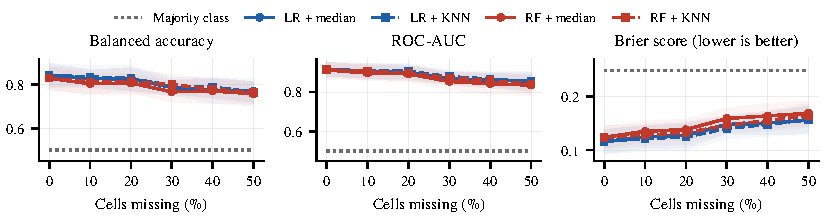
\includegraphics[width=\linewidth]{figures/fig_performance.pdf}
  \caption{Performance as feature values are removed (matched scenario; mean of 15 splits, shading $\pm1$ SD; dotted: majority-class baseline).}
  \label{fig:perf}
\end{figure}
\textbf{Baseline and models.} The majority-class baseline scores balanced accuracy 0.500, AUC 0.500, Brier 0.248; on complete data LR with median imputation reaches 0.844, 0.916, 0.116; at 50\% missing cells, 0.771, 0.857 and 0.156. The decline is gradual (Fig.~\ref{fig:perf}) and every model stays far above the baseline. RF is not better: its paired balanced-accuracy difference from LR is between $-0.023$ and $+0.005$ at all levels, it wins in only 13--47\% of splits, and it is slightly worse in AUC and Brier score in all 12 level--imputer combinations. KNN beats median imputation by at most 0.033, within the run-to-run SD.

\begin{table}[t]
  \caption{Selective prediction, 80\% target coverage (mean of 15 splits; SD: coverage 0.07--0.09, risks 0.04--0.07). ``All'': error without abstention. Last column: coverage at 50\% missing, clean training and $\tau$.}
  \label{tab:sel}
  \centering
  \footnotesize
  \setlength{\tabcolsep}{4pt}
  \begin{tabular}{lccc|ccc|c}
    \toprule
    & \multicolumn{3}{c|}{0\% missing} & \multicolumn{3}{c|}{50\% missing} & 50\%, clean\\
    Model & Cov. & Sel. risk & All & Cov. & Sel. risk & All & threshold: Cov.\\
    \midrule
    LR + median & 0.77 & 0.112 & 0.158 & 0.79 & 0.173 & 0.231 & 0.67\\
    LR + KNN    & 0.77 & 0.106 & 0.157 & 0.78 & 0.155 & 0.219 & 0.77\\
    RF + median & 0.79 & 0.113 & 0.166 & 0.79 & 0.205 & 0.260 & 0.73\\
    RF + KNN    & 0.78 & 0.112 & 0.165 & 0.77 & 0.180 & 0.244 & 0.84\\
    \bottomrule
  \end{tabular}
\end{table}
\textbf{Selective prediction.} Skipping about a fifth of patients lowers the error among answered patients in all 24 model--imputer--level settings (Table~\ref{tab:sel}), for example from 0.158 to 0.112 for LR with median imputation on complete data. The mean reduction is 0.034--0.073 and does not shrink as data go missing, but it does not undo the damage: at 50\% missing the selective risk (0.155--0.205) exceeds the complete-data error without abstention (0.157--0.166) in three of four configurations.

\textbf{Which errors, and who is skipped?} For LR with median imputation the false-negative rate (missed disease) rises from 0.20 to 0.29 between 0 and 50\% missing; missed disease is 52--61\% of all errors. Abstention is selective but far from complete: LR skips 44\% of its wrong but only 19\% of its correct predictions on complete data, so over half its mistakes are answered. The eight most confident errors of patients misclassified in all three test appearances at 0\% missing (33 patients, 10.9\%) are five diseased patients who look low-risk on every recorded feature (no exercise angina, no coloured vessels, normal thal, ST depression 0; predicted probability 0.04--0.14) and three healthy patients with a reversible thal defect and one to three coloured vessels (0.90--0.94); none was ever skipped. No confidence threshold can catch such confident mistakes.

\section{Graduate Depth Analysis}
\begin{figure}[t]
  \centering
  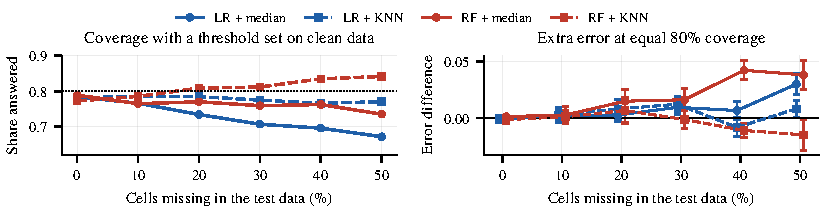
\includegraphics[width=\linewidth]{figures/fig_failure_audit.pdf}
  \caption{Failure-mode audit. Left: coverage when training, tuning and $\tau$ use clean data and only test rows are incomplete (dotted: 80\% target). Right: extra error at equal 80\% coverage versus the matched scenario ($\pm1$ standard error).}
  \label{fig:audit}
\end{figure}
\textbf{Failure-mode audit.} A team would typically choose $\tau$ once, on clean data, and then deploy the model where records are incomplete. Does the threshold still deliver the promised coverage? We keep training, tuning and validation data clean, mask only test rows, and report coverage and the error among the 80\% most confident test predictions.

\textbf{Findings.} With median imputation the planned coverage is not met (Fig.~\ref{fig:audit}): LR coverage falls from 0.78 to 0.67 at 50\% missing (0.79 with the matched threshold; lower in 14 of 15 splits), RF from 0.79 to 0.73. With KNN, LR shows no consistent change while RF answers \emph{more} than planned (0.84, $+0.070$). At equal coverage the clean-trained median models are slightly worse at 50\% missing (LR $+0.030$, RF $+0.038$). The main failure is thus lost or surplus coverage, not a jump in the error of answered cases.

\textbf{What this teaches.} A system audited only on accuracy could silently answer 12 percentage points fewer patients than intended (67\% instead of 79\%). Thresholds should be set on validation data whose missingness resembles deployment, with coverage monitored in use.

\section{Limitations and Conclusion}
The most important limitation is that missingness is simulated completely at random; real missingness depends on the patient, so absolute numbers should not be carried over. A stronger claim would need multi-site data with recorded missingness, non-random simulations, external validation and prospective evaluation. Further limits: 303 patients from one site, so coverage varies by $\pm$0.07--0.09 between splits and balanced-accuracy gaps below about 0.03 are unresolved; selective models see 75\% of each training fold; a binary target that merges severities; and the assumption that all measurements exist at prediction time. The features are predictive indicators, not causes.

\textbf{Conclusion.} Missing values degrade reliability gradually (from 0 to 50\% missing, LR balanced accuracy falls about 0.07 and AUC about 0.06) and a random forest does not help. Abstaining on the least confident 20\% of patients lowers error on the rest by about 0.05 at every level without restoring complete-data performance, and a threshold set on clean data does not transfer reliably.

\section{Reproducibility and AI-Use Disclosure}
\textbf{Code and data.} The data are public at \url{https://archive.ics.uci.edu/dataset/45/heart+disease}. The submitted archive holds the raw Cleveland file, all code, saved results, fixed seeds, pinned package versions and a walkthrough notebook. \texttt{bash run\_all.sh} regenerates every table and figure in about 20 minutes on one CPU core. No private data, passwords or API keys are used.

\textbf{AI-use disclosure.} I used Claude (Anthropic) as a coding and writing assistant: to write and debug the Python pipeline, run the experiments, make the figures, and draft and edit this text. Checks: I ran the six automated leakage tests on my own computer (all pass); the assisted workflow also checked the converted data against the raw UCI file and every quoted number against the saved results. I remain responsible for the work and can explain it.

\setlength{\bibsep}{0pt}
\begin{thebibliography}{99}\small
\bibitem[Breiman(2001)]{breiman2001}
L.~Breiman. Random forests. \emph{Machine Learning}, 45(1):5--32, 2001.

\bibitem[Detrano et al.(1989)]{detrano1989}
R.~Detrano et al. International application of a new probability algorithm for the diagnosis of coronary artery disease. \emph{American Journal of Cardiology}, 64(5):304--310, 1989.

\bibitem[El-Yaniv and Wiener(2010)]{elyaniv2010}
R.~El-Yaniv and Y.~Wiener. On the foundations of noise-free selective classification. \emph{Journal of Machine Learning Research}, 11:1605--1641, 2010.

\bibitem[Janosi et al.(1988)]{uci}
A.~Janosi et al. Heart Disease. UCI Machine Learning Repository, 1988. \url{https://archive.ics.uci.edu/dataset/45/heart+disease}.

\bibitem[Kapoor and Narayanan(2023)]{kapoor2023}
S.~Kapoor and A.~Narayanan. Leakage and the reproducibility crisis in machine-learning-based science. \emph{Patterns}, 4(9):100804, 2023.

\bibitem[Pedregosa et al.(2011)]{pedregosa2011}
F.~Pedregosa et al. Scikit-learn: Machine learning in Python. \emph{Journal of Machine Learning Research}, 12:2825--2830, 2011.

\bibitem[Troyanskaya et al.(2001)]{troyanskaya2001}
O.~Troyanskaya et al. Missing value estimation methods for DNA microarrays. \emph{Bioinformatics}, 17(6):520--525, 2001.
\end{thebibliography}

\end{document}
